\documentclass{beamer}
\usetheme{Boadilla}
\usecolortheme{default}
\usepackage[utf8]{inputenc}
\usepackage{amsmath}
\usepackage{amsfonts}
\usepackage{amssymb}
\usepackage{amsthm}
\usepackage{array}
\usepackage{float}
\usepackage{listings}
\usepackage{color}
\usepackage{caption}
\usepackage{multirow}
\usepackage{caption}
\usepackage{subcaption}
\usepackage{multimedia}
\usepackage{tikz}
\usetikzlibrary{shapes.misc,shadows}
\usetikzlibrary{quotes,positioning,arrows,decorations.markings}
\usetikzlibrary{positioning} 
\usepackage[cache=true,section]{minted}
%\usepackage[a4paper, total={6in, 8in}]{geometry}
\usepackage[tworuled,algosection,figure,linesnumbered]{algorithm2e}
\usepackage{glossaries}
\usemintedstyle{default}
\newminted{haskell}{frame=lines,framerule=2pt}
\newminted{R}{frame=lines,framerule=2pt}
\graphicspath{{./images/}}
\newcommand{\DP}{\mathsf{DP}}
\newcommand{\dpwcc}{\mathsf{DP_{WCC}}}
\newcommand{\iwcc}{\mathsf{Sr}}
\newcommand{\iwc}{\mathsf{Sr_{WCC}}}
\newcommand{\owcc}{\mathsf{Sk}}
\newcommand{\owc}{\mathsf{Sk_{WCC}}}
\newcommand{\fwcc}{\mathsf{F}} 
\newcommand{\fwc}{\mathsf{F_{WCC}}} 
\newcommand{\gwcc}{\mathsf{G}}
\newcommand{\gwc}{\mathsf{G_{WCC}}}
\newcommand{\ice}{\mathsf{IC_E}}
\newcommand{\csofv}{\mathsf{IC_{set(V)}}}
\newcommand{\sgen}{\mathsf{S_G}}
\newcommand{\sfilter}{\mathsf{S_F}}
\newcommand{\sinp}{\mathsf{S_I}}
\newcommand{\sout}{\mathsf{S_O}}
\newcommand{\istream}{\mathsf{D}}
\newcommand{\wccout}{\mathsf{R}}
\newcommand{\fmem}{\mathsf{M_F}}
\newcommand{\eof}{\mathsf{eof}}
\newcommand{\Act}{\mathsf{actor_1}}
\newcommand{\Actt}{\mathsf{actor_2}}
\definecolor{androidgreen}{rgb}{0.64,0.78,0.22}
\definecolor{titaniumyellow}{rgb}{0.93,0.9,0.0}
\definecolor{light}{rgb}{0.5, 0.5, 0.5}

\makeatletter
\long\def\beamer@author[#1]#2{%
  \def\insertauthor{\def\inst{\beamer@insttitle}\def\and{\beamer@andtitle}%
  \begin{tabular}{rl}#2\end{tabular}}%
  \def\beamer@shortauthor{#1}%
  \ifbeamer@autopdfinfo%
    \def\beamer@andstripped{}%
    \beamer@stripands#1 \and\relax
    {\let\inst=\@gobble\let\thanks=\@gobble\def\and{, }\hypersetup{pdfauthor={\beamer@andstripped}}}
  \fi%
}
\makeatother

\makeatletter
\pgfdeclareshape{datastore}{
  \inheritsavedanchors[from=rectangle]
  \inheritanchorborder[from=rectangle]
  \inheritanchor[from=rectangle]{center}
  \inheritanchor[from=rectangle]{base}
  \inheritanchor[from=rectangle]{north}
  \inheritanchor[from=rectangle]{north east}
  \inheritanchor[from=rectangle]{east}
  \inheritanchor[from=rectangle]{south east}
  \inheritanchor[from=rectangle]{south}
  \inheritanchor[from=rectangle]{south west}
  \inheritanchor[from=rectangle]{west}
  \inheritanchor[from=rectangle]{north west}
  \backgroundpath{
    %  store lower right in xa/ya and upper right in xb/yb
    \southwest \pgf@xa=\pgf@x \pgf@ya=\pgf@y
    \northeast \pgf@xb=\pgf@x \pgf@yb=\pgf@y
    \pgfpathmoveto{\pgfpoint{\pgf@xa}{\pgf@ya}}
    \pgfpathlineto{\pgfpoint{\pgf@xb}{\pgf@ya}}
    \pgfpathmoveto{\pgfpoint{\pgf@xa}{\pgf@yb}}
    \pgfpathlineto{\pgfpoint{\pgf@xb}{\pgf@yb}}
 }
}
\makeatother

\title[Incrementally Enumerating BT in BG]{An Algorithm for incrementally Enumerating Bitriangles in large Bipartite Networks}
\subtitle{Master Thesis\vspace{-0.5cm}}
\author[Juan Pablo Royo Sales (Master Thesis)]{\vspace{-0.5cm}Juan Pablo Royo Sales}
\institute[]{%
  {\small Facultat d’Informàtica de Barcelona (FIB)}\\
  {\small Universitat Politècnica de Catalunya (UPC) – BarcelonaTech}\\
  \vspace{0.2cm}
  Master in Innovation and Research in Informatics\\ 
  Advance Computing\\
  \vspace{0.2cm}
  \tiny{%
  Supervisors: Edelmira Pasarella, Computer Science Department\\
  Maria-Esther Vidal, Leibniz Information Centre for Science and Technology-TIB, and L3S Centre at the Leibniz University of Hannover\\
  Cristina Zoltan, Computer Science Department
  }
}

\date[October 29, 2021]{October 29, 2021}
  
\titlegraphic{%
  \begin{tikzpicture}[overlay,remember picture]
    \node[left=3.5cm] at (current page.30){
      
\includegraphics[height=1.5cm]{upc_logo}
    };
  \end{tikzpicture}
}

\usetikzlibrary{external,quotes,positioning,calc,arrows,decorations.markings,positioning,fit,shapes.misc,shadows}

\newcommand{\inputtikz}[1]{%
  \tikzsetnextfilename{#1}%
  \input{tikz/#1.tikz}
}

\tikzexternalize[shell escape=-shell-escape,mode=graphics if exists,prefix=images/]
\begin{document}

  \begin{frame}
    \vspace{1.3cm}
    \titlepage
  \end{frame}

  \begin{frame}{Agenda}
    \tableofcontents
  \end{frame}
  
  \begin{frame}{Agenda}
    \section{Motivation}
    \tableofcontents[currentsection]
  \end{frame}

  \begin{frame}[fragile]{Motivation}
    \begin{center}
      Provide an Algorithm for Incrementally Enumarting Bitriangles in large Bipartite Networks using \textbf{Dynamic Pipeline Paradigm}
    \end{center}    
  \end{frame}

  \begin{frame}[fragile]{Motivation}
    \begin{center}
      {\color{light}Provide an Algorithm for Incrementally Enumarting Bitriangles in large} \underline{{\color{red}\textbf{Bipartite Networks}}} {\color{light}{using \textbf{Dynamic Pipeline Paradigm}}}
    \end{center}    
    \vspace{0.5cm}
    \begin{tikzpicture}[overlay, remember picture]
      \node[yshift=3cm] at (current page.south) {
        \inputtikz{bipartite}
      };
    \end{tikzpicture}
  \end{frame}

  \begin{frame}[fragile]{Motivation}
    \begin{center}
      {\color{light}Provide an Algorithm for Incrementally Enumarting} \underline{{\color{red}\textbf{Bitriangles}}} {\color{light}{in large Bipartite Networks using \textbf{Dynamic Pipeline Paradigm}}}
    \end{center}    
    \vspace{0.5cm}
    \begin{tikzpicture}[overlay, remember picture]
      \node[yshift=3cm] at (current page.south) {
        \inputtikz{bitriangle}
      };
    \end{tikzpicture}
  \end{frame}


  \begin{frame}[fragile]{Motivation}
    \begin{center}
      Provide an Algorithm for Incrementally Enumarting Bitriangles in large Bipartite Networks using \textbf{Dynamic Pipeline Paradigm}
    \end{center}    
    \vspace{0.5cm}
    \begin{center}
    \huge\emph{Why?}
    \end{center}
  \end{frame}

  \begin{frame}[fragile]{Motivation}
    \begin{center}
      Provide an Algorithm for Incrementally Enumarting Bitriangles in large Bipartite Networks using \textbf{Dynamic Pipeline Paradigm}
    \end{center}    
    \begin{block}{Why?}
      \begin{itemize}
        \item Bipartite graph model interesting relations between different set of objects, i.e. \textbf{phenotype-disease gene associations network, Netflix subscribers-TV shows, author-papers, etc.}
      \end{itemize}
    \end{block}
  \end{frame}

  \begin{frame}[fragile]{Motivation}
    \begin{center}
      Provide an Algorithm for Incrementally Enumarting Bitriangles in large Bipartite Networks using \textbf{Dynamic Pipeline Paradigm}
    \end{center}    
    \begin{block}{Why?}
      \begin{itemize}
        \item {\color{light}Bipartite graph model interesting relations between different set of objects, i.e. \textbf{phenotype-disease gene associations network, Netflix subscribers-TV shows, author-papers, etc.}}
        \item Metrics for analyzing relations \textbf{Clustering coefficient, communities, social analysis}, based on Bitriangles amount.
      \end{itemize}
    \end{block}
  \end{frame}

  \begin{frame}[fragile]{Motivation}
    \begin{center}
      Provide an Algorithm for Incrementally Enumarting Bitriangles in large Bipartite Networks using \textbf{Dynamic Pipeline Paradigm}
    \end{center}    
    \begin{block}{Why?}
      \begin{itemize}
        \item {\color{light}Bipartite graph model interesting relations between different set of objects, i.e. \textbf{phenotype-disease gene associations network, Netflix subscribers-TV shows, author-papers, etc.}}
        \item {\color{light}Metrics for analyzing relations \textbf{Clustering coefficient, communities, social analysis}, based on Bitriangles amount.}
        \item Counting is \textbf{not enough}. Needs to know structural components of bitriangles, for example: in diseasome netowrk 2 disorders are connected if there is a gene implicated in both. 
      \end{itemize}
    \end{block}
  \end{frame}

  \begin{frame}[fragile]{Motivation}
    \begin{center}
      Provide an Algorithm for Incrementally Enumarting Bitriangles in large Bipartite Networks using \textbf{Dynamic Pipeline Paradigm}
    \end{center}    
    \begin{block}{Why?}
      \begin{itemize}
        \item {\color{light}Bipartite graph model interesting relations between different set of objects, i.e. \textbf{phenotype-disease gene associations network, Netflix subscribers-TV shows, author-papers, etc.}}
        \item {\color{light}Metrics for analyzing relations \textbf{Clustering coefficient, communities, social analysis}, based on Bitriangles amount.}
        \item {\color{light}Counting is \textbf{not enough}. Needs to know structural components of bitriangles, for example: in diseasome netowrk 2 disorders are connected if there is a gene implicated in both.}
        \item \emph{"All-or-Nothing" vs. "Pay-as-you-go"} model: Some results are enough to conduct analysis like in diseasome netowrks. 
      \end{itemize}
    \end{block}
  \end{frame}

  \begin{frame}[fragile]{Motivation}
    \begin{center}
      Provide an Algorithm for Incrementally Enumarting Bitriangles in large Bipartite Networks using \textbf{Dynamic Pipeline Paradigm}
    \end{center}    
    \vspace{0.5cm}
    \begin{center}
      \huge\emph{How?}
    \end{center}  
  \end{frame}

  \begin{frame}[fragile]{Motivation}
    \begin{center}
      Provide an Algorithm for Incrementally Enumarting Bitriangles in large Bipartite Networks using \textbf{Dynamic Pipeline Paradigm}
    \end{center}    
    \begin{block}{How?}
      \begin{itemize}
        \item Provide a \textbf{Proof of Concept} to test \textbf{Haskell} suitability for implementing  \textbf{Dynamic Pipeline Paradigm} solving Weakly Connected Components Problem
    \end{itemize}   
  \end{block} 
  \end{frame}

  \begin{frame}[fragile]{Motivation}
    \begin{center}
      Provide an Algorithm for Incrementally Enumarting Bitriangles in large Bipartite Networks using \textbf{Dynamic Pipeline Paradigm}
    \end{center}    
    \begin{block}{How?}
      \begin{itemize}
        \item {\color{light}Provide a \textbf{Proof of Concept} to test \textbf{Haskell} suitability for implementing  \textbf{Dynamic Pipeline Paradigm} solving Weakly Connected Components Problem}
        \item Build a \textbf{Dynamic Pipeline Framework} in \textbf{Haskell} to implement any algorithm 
    \end{itemize}   
  \end{block} 
  \end{frame}

  \begin{frame}[fragile]{Motivation}
    \begin{center}
      Provide an Algorithm for Incrementally Enumarting Bitriangles in large Bipartite Networks using \textbf{Dynamic Pipeline Paradigm}
    \end{center}    
    \begin{block}{How?}
      \begin{itemize}
        \item {\color{light}Provide a \textbf{Proof of Concept} to test \textbf{Haskell} suitability for implementing  \textbf{Dynamic Pipeline Paradigm} solving Weakly Connected Components Problem}
        \item {\color{light}Build a \textbf{Dynamic Pipeline Framework} in \textbf{Haskell} to implement any algorithm }
        \item Provide an pseudo-code algorithm definition for \textbf{Incrementally Enumerating Bitriangles in large Bipartite Networks}
    \end{itemize}   
  \end{block} 
  \end{frame}

  \begin{frame}[fragile]{Motivation}
    \begin{center}
      Provide an Algorithm for Incrementally Enumarting Bitriangles in large Bipartite Networks using \textbf{Dynamic Pipeline Paradigm}
    \end{center}    
    \begin{block}{How?}
      \begin{itemize}
        \item {\color{light}Provide a \textbf{Proof of Concept} to test \textbf{Haskell} suitability for implementing  \textbf{Dynamic Pipeline Paradigm} solving Weakly Connected Components Problem}
        \item {\color{light}Build a \textbf{Dynamic Pipeline Framework} in \textbf{Haskell} to implement any algorithm }
        \item {\color{light}Provide an pseudo-code algorithm definition for \textbf{Incrementally Enumerating Bitriangles in large Bipartite Networks}}
        \item Implement that Algorithm using \textbf{Dynamic Pipeline Framework in Haskell}
    \end{itemize}   
  \end{block} 
  \end{frame}


  \begin{frame}{Agenda}
    \section{Dynamic Pipeline Paradigm}
    \tableofcontents[currentsection]
  \end{frame}

  \inputtikz{genericDP-Fig}
  \begin{frame}[fragile]{Dynamic Pipeline Paradigm}
    \begin{tikzpicture}[overlay, remember picture]
      \node[xshift=-3cm,yshift=-2cm] at (current page.north east) {
        \inputtikz{graph-DP-Fig}
      };
    \end{tikzpicture}
    \begin{figure}
      \centering
      \resizebox{\textwidth}{!}{\inputtikz{dp_example_0}}
    \end{figure}
  \end{frame}

  \begin{frame}[fragile]{Dynamic Pipeline Paradigm}
    \begin{tikzpicture}[overlay, remember picture]
      \node[xshift=-1.5cm,yshift=-0.7cm] at (current page.north east) {
        \resizebox{2cm}{1cm}{\inputtikz{graph-DP-Fig}}
      };
      \node[xshift=3cm,yshift=-2cm,opacity=0.3] at (current page.north west) {
        \resizebox{5cm}{2cm}{\inputtikz{dp_example_0}}
      };
    \end{tikzpicture}
    \begin{figure}
      \centering
      \resizebox{\textwidth}{!}{\inputtikz{dp_example_1}}
    \end{figure}
  \end{frame}

  \begin{frame}[fragile]{Dynamic Pipeline Paradigm}
    \begin{tikzpicture}[overlay, remember picture]
      \node[xshift=-1.5cm,yshift=-0.7cm] at (current page.north east) {
        \resizebox{2cm}{1cm}{\inputtikz{graph-DP-Fig}}
      };
    \node[xshift=3cm,yshift=-2cm,opacity=0.3] at (current page.north west) {
      \resizebox{5cm}{2cm}{\inputtikz{dp_example_0}}
      };
    \node[xshift=9cm,yshift=-2cm,opacity=0.3] at (current page.north west) {
        \resizebox{6cm}{2cm}{\inputtikz{dp_example_1}}
    };
  \end{tikzpicture}
    \begin{figure}
      \centering
      \resizebox{\textwidth}{!}{\inputtikz{dp_example_2}}
    \end{figure}
  \end{frame}   

  \begin{frame}[fragile]{Dynamic Pipeline Paradigm}
    \begin{tikzpicture}[overlay, remember picture]
      \node[xshift=-1.5cm,yshift=-0.7cm] at (current page.north east) {
        \resizebox{2cm}{1cm}{\inputtikz{graph-DP-Fig}}
      };
      \node[xshift=3cm,yshift=-2cm,opacity=0.3] at (current page.north west) {
        \resizebox{5cm}{2cm}{\inputtikz{dp_example_1}}
        };
      \node[xshift=9cm,yshift=-2cm,opacity=0.3] at (current page.north west) {
          \resizebox{6cm}{2cm}{\inputtikz{dp_example_2}}
      };
    \end{tikzpicture}
    \begin{figure}
      \centering
      \resizebox{\textwidth}{!}{\inputtikz{dp_example_3}}
    \end{figure}
  \end{frame}   

  \begin{frame}[fragile]{Dynamic Pipeline Paradigm}
    \begin{tikzpicture}[overlay, remember picture]
      \node[xshift=-1.5cm,yshift=-0.7cm] at (current page.north east) {
        \resizebox{2cm}{1cm}{\inputtikz{graph-DP-Fig}}
      };
      \node[xshift=3cm,yshift=-2cm,opacity=0.3] at (current page.north west) {
        \resizebox{5cm}{2cm}{\inputtikz{dp_example_2}}
        };
      \node[xshift=9cm,yshift=-2cm,opacity=0.3] at (current page.north west) {
          \resizebox{6cm}{2cm}{\inputtikz{dp_example_3}}
      };
    \end{tikzpicture}
    \begin{figure}
      \centering
      \resizebox{\textwidth}{!}{\inputtikz{dp_example_4}}
    \end{figure}
  \end{frame}   

  \begin{frame}[fragile]{Dynamic Pipeline Paradigm}
    \begin{tikzpicture}[overlay, remember picture]
      \node[xshift=-1.5cm,yshift=-0.7cm] at (current page.north east) {
        \resizebox{2cm}{1cm}{\inputtikz{graph-DP-Fig}}
      };
      \node[xshift=3cm,yshift=-2cm,opacity=0.3] at (current page.north west) {
        \resizebox{5cm}{2cm}{\inputtikz{dp_example_3}}
        };
      \node[xshift=9cm,yshift=-2cm,opacity=0.3] at (current page.north west) {
          \resizebox{6cm}{2cm}{\inputtikz{dp_example_4}}
      };
    \end{tikzpicture}
    \begin{figure}
      \centering
      \resizebox{\textwidth}{!}{\inputtikz{dp_example_5}}
    \end{figure}
  \end{frame}   

  \begin{frame}[fragile]{Dynamic Pipeline Paradigm}
    \begin{tikzpicture}[overlay, remember picture]
      \node[xshift=-1.5cm,yshift=-0.7cm] at (current page.north east) {
        \resizebox{2cm}{1cm}{\inputtikz{graph-DP-Fig}}
      };
      \node[xshift=3cm,yshift=-2cm,opacity=0.3] at (current page.north west) {
        \resizebox{5cm}{2cm}{\inputtikz{dp_example_4}}
        };
      \node[xshift=9cm,yshift=-2cm,opacity=0.3] at (current page.north west) {
          \resizebox{6cm}{2cm}{\inputtikz{dp_example_5}}
      };
    \end{tikzpicture}
    \begin{figure}
      \centering
      \resizebox{\textwidth}{!}{\inputtikz{dp_example_6}}
    \end{figure}
  \end{frame}  

  \begin{frame}[fragile]{Dynamic Pipeline Paradigm}
    \begin{tikzpicture}[overlay, remember picture]
      \node[xshift=-1.5cm,yshift=-0.7cm] at (current page.north east) {
        \resizebox{2cm}{1cm}{\inputtikz{graph-DP-Fig}}
      };
      \node[xshift=3cm,yshift=-2cm,opacity=0.3] at (current page.north west) {
        \resizebox{5cm}{2cm}{\inputtikz{dp_example_5}}
        };
      \node[xshift=9cm,yshift=-2cm,opacity=0.3] at (current page.north west) {
          \resizebox{6cm}{2cm}{\inputtikz{dp_example_6}}
      };
    \end{tikzpicture}
    \begin{figure}
      \centering
      \inputtikz{dp_example_7}
    \end{figure}
  \end{frame}  

  \begin{frame}[fragile]{Dynamic Pipeline Paradigm}
    \begin{tikzpicture}[overlay, remember picture]
      \node[xshift=-1.5cm,yshift=-0.7cm] at (current page.north east) {
        \resizebox{2cm}{1cm}{\inputtikz{graph-DP-Fig}}
      };
      \node[xshift=3cm,yshift=-2cm,opacity=0.3] at (current page.north west) {
        \resizebox{5cm}{2cm}{\inputtikz{dp_example_6}}
        };
      \node[xshift=9cm,yshift=-2cm,opacity=0.3] at (current page.north west) {
          \resizebox{6cm}{2cm}{\inputtikz{dp_example_7}}
      };
    \end{tikzpicture}
    \begin{figure}
      \centering
      \inputtikz{dp_example_8}
    \end{figure}
  \end{frame} 
  
  \begin{frame}[fragile]{Dynamic Pipeline Paradigm}
    \begin{tikzpicture}[overlay, remember picture]
      \node[xshift=-1.5cm,yshift=-0.7cm] at (current page.north east) {
        \resizebox{2cm}{1cm}{\inputtikz{graph-DP-Fig}}
      };
      \node[xshift=3cm,yshift=-2cm,opacity=0.3] at (current page.north west) {
        \resizebox{5cm}{2cm}{\inputtikz{dp_example_7}}
        };
      \node[xshift=9cm,yshift=-2cm,opacity=0.3] at (current page.north west) {
          \resizebox{6cm}{2cm}{\inputtikz{dp_example_8}}
      };
    \end{tikzpicture}
    \begin{figure}
      \centering
      \inputtikz{dp_example_9}
    \end{figure}
  \end{frame}  

  \begin{frame}[fragile]{Dynamic Pipeline Paradigm}
    \begin{tikzpicture}[overlay, remember picture]
      \node[xshift=-1.5cm,yshift=-0.7cm] at (current page.north east) {
        \resizebox{2cm}{1cm}{\inputtikz{graph-DP-Fig}}
      };
      \node[xshift=3cm,yshift=-2cm,opacity=0.3] at (current page.north west) {
        \resizebox{5cm}{2cm}{\inputtikz{dp_example_8}}
        };
      \node[xshift=9cm,yshift=-2cm,opacity=0.3] at (current page.north west) {
          \resizebox{6cm}{1cm}{\inputtikz{dp_example_9}}
      };
    \end{tikzpicture}
    \begin{figure}
      \centering
      \inputtikz{dp_example_10}
    \end{figure}
  \end{frame}  

  \begin{frame}[fragile]{Dynamic Pipeline Paradigm}
    \begin{tikzpicture}[overlay, remember picture]
      \node[xshift=-1.5cm,yshift=-0.7cm] at (current page.north east) {
        \resizebox{2cm}{1cm}{\inputtikz{graph-DP-Fig}}
      };
      \node[xshift=3cm,yshift=-2cm,opacity=0.3] at (current page.north west) {
        \resizebox{5cm}{1cm}{\inputtikz{dp_example_9}}
        };
      \node[xshift=9cm,yshift=-2cm,opacity=0.3] at (current page.north west) {
          \resizebox{5cm}{1cm}{\inputtikz{dp_example_10}}
      };
    \end{tikzpicture}
    \begin{figure}
      \centering
      \inputtikz{dp_example_11}
    \end{figure}
  \end{frame}  

  \begin{frame}[fragile]{Dynamic Pipeline Paradigm}
    \begin{tikzpicture}[overlay, remember picture]
      \node[xshift=-1.5cm,yshift=-0.7cm] at (current page.north east) {
        \resizebox{2cm}{1cm}{\inputtikz{graph-DP-Fig}}
      };
      \node[xshift=3cm,yshift=-2cm,opacity=0.3] at (current page.north west) {
        \resizebox{5cm}{1cm}{\inputtikz{dp_example_10}}
        };
      \node[xshift=9cm,yshift=-2cm,opacity=0.3] at (current page.north west) {
          \resizebox{5cm}{1cm}{\inputtikz{dp_example_11}}
      };
    \end{tikzpicture}
    \begin{figure}
      \centering
      \inputtikz{dp_example_12}
    \end{figure}
  \end{frame}  

  \begin{frame}{Agenda}
    \section{Proof of Concept: $DP_{WCC}$}
    \tableofcontents[currentsection]
  \end{frame}

  \begin{frame}[fragile]{Proof of Concept: $DP_{WCC}$}
    \begin{block}{Summary}
    \begin{itemize}
      \item Develop the algorithm presented before using \textbf{Haskell}
    \end{itemize}
    \end{block}
  \end{frame}

  \begin{frame}[fragile]{Proof of Concept: $DP_{WCC}$}
    \begin{block}{Summary}
    \begin{itemize}
      \item {\color{light}Develop the algorithm presented before using \textbf{Haskell}}
      \item Conduct empirical analysis to prove suitability of implementation
    \end{itemize}
    \end{block}
  \end{frame}

  \begin{frame}[fragile]{Proof of Concept: $DP_{WCC}$}
    \begin{block}{Summary}
    \begin{itemize}
      \item {\color{light}Develop the algorithm presented before using \textbf{Haskell}}
      \item {\color{light}Conduct empirical analysis to prove suitability of implementation}
      \item Write an \textbf{article} and present the results in \textbf{PROLE21 Conference}~\cite{prole:2021:017}
    \end{itemize}
    \end{block}
  \end{frame}
  
  \begin{frame}[fragile]{Proof of Concept: $DP_{WCC}$ - Empirical Evaluation}
    \begin{block}{Research Questions}
      \begin{itemize}
            \item Does $\dpwcc$ in Haskell support the dynamic parallelization level that $\dpwcc$ requires?
            \item Is $\dpwcc$ in Haskell competitive compared with default implementations on base libraries for the same problem?
            \item Does $\dpwcc$ in Haskell handle memory efficiently?
        \end{itemize}        
    \end{block}
    \begin{block}{Experiments}
      \begin{itemize}
        \item \textbf{Implementation Analysis}: Measure and analyze Total execution time, MUT time and GC Time.
        \item \textbf{Benchmark Analysis}: Compare $DP_{WCC}$ with \mintinline{haskell}{Data.Graph} $WCC$ execution times:
        \begin{itemize}
          \item Using \mintinline{haskell}{ criterion } library.
          \item Diefficency metric $\mathtt{dief@t}$ (\textit{diepfy} tool) to measure incremental results.
        \end{itemize}
        \item \textbf{Performance Analysis}: Thread and Memory allocation analysis.
      \end{itemize}
    \end{block}
  \end{frame}

  \begin{frame}[fragile]{Proof of Concept: $DP_{WCC}$ - Conclusions}
    \begin{block}{Conclusions}      

    \begin{itemize}
      \item \textbf{Robustness and Suitability} of the DP-Haskell 
      \item \textbf{Ability to generate Incremental results} has been shown by $\mathtt{dief@t}$ metrics
      \item \textbf{Satisfactory Performance results} with an adequate Memory allocation and Execution times. 
    \end{itemize}
  \end{block}
  \end{frame}


  \begin{frame}{Agenda}
    \section{DP Haskell Framework}
    \tableofcontents[currentsection]
  \end{frame}

  \begin{frame}[fragile]{DP Haskell Framework}
    \begin{center}
      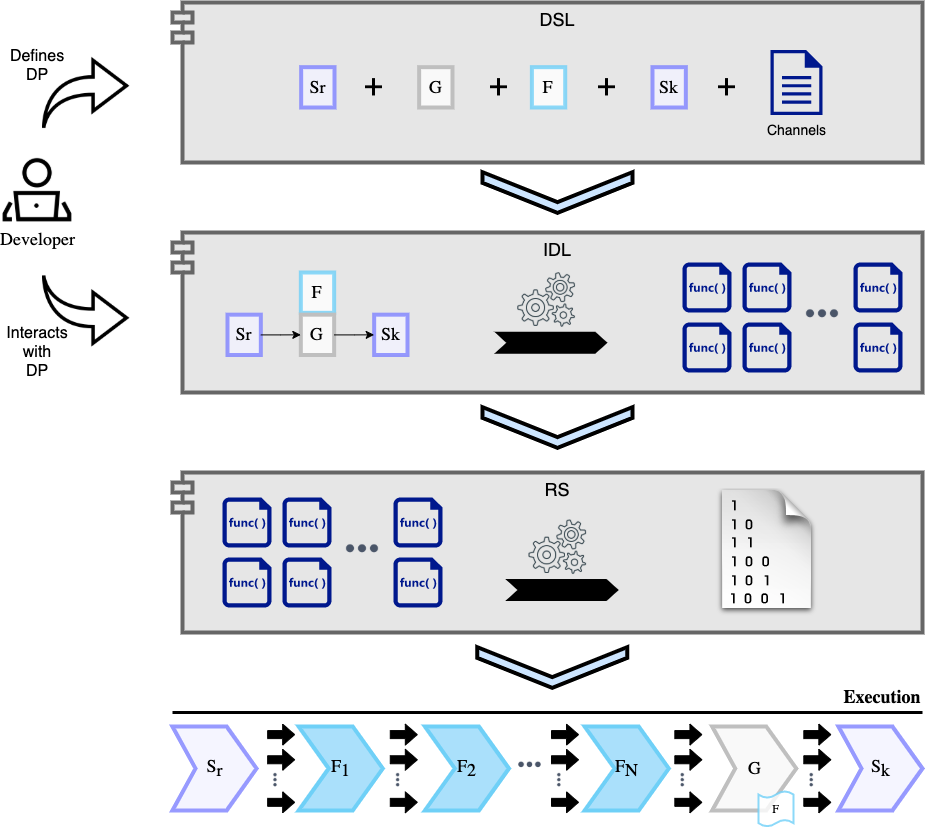
\includegraphics[width = 0.8\textwidth, height = 0.8\textheight]{dpf_haskell_v3}
    \end{center}
  \end{frame}

    \begin{frame}[fragile]{DP Haskell Framework}
      \begin{center}
      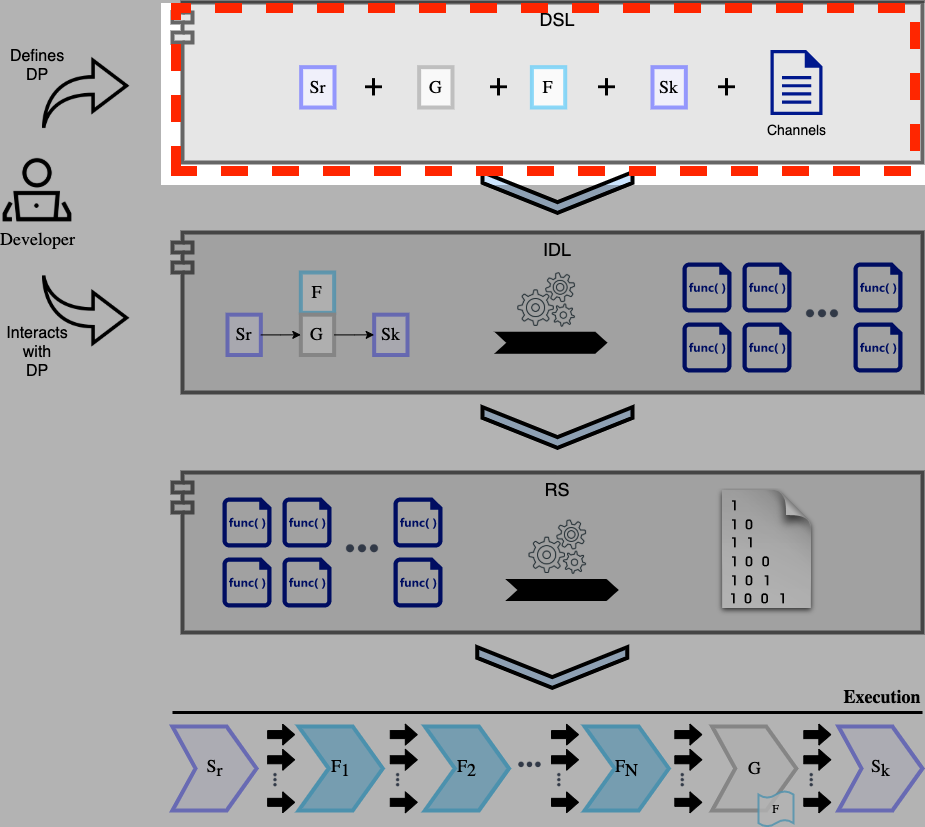
\includegraphics[width = 0.8\textwidth, height = 0.8\textheight]{dpf_haskell_v3-1}
    \end{center}
  \end{frame}

  \lstset{
    basicstyle=\itshape,
    literate={->}{$\rightarrow$}{2}
  }

  \begin{frame}[fragile]{DP Haskell Framework}
    \frametitle{DSL Grammar}
    \small
    \begin{equation*}
      \boxed{
       \begin{aligned}
      G_{dsl} = (N, \Sigma, DB, P)
      \end{aligned}
      }
  \end{equation*}
  \tiny
      \begin{equation*}
          \boxed{
           \begin{aligned}
          N &= \{DP,S_r,S_k,G,F_b,CH,CH_s\},\\
          \Sigma &= \{\text{\mintinline{haskell}{Source}},\text{\mintinline{haskell}{Generator}},\text{\mintinline{haskell}{Sink}},\text{\mintinline{haskell}{FeedbackChannel}},\text{\mintinline{haskell}{Type}},\text{\mintinline{haskell}{Eof}},\text{\mintinline{haskell}{:=>}},\text{\mintinline{haskell}{:<+>}}\},
          \end{aligned}
          }
      \end{equation*}
    \small
    \begin{equation*}
      \boxed{
        \begin{aligned}
      P = \{\\
      DP  &\rightarrow S_r\ \text{\mintinline{haskell}{:=>}}\ G\ \text{\mintinline{haskell}{:=>}}\ S_k\ |\ S_r\ \text{\mintinline{haskell}{:=>}}\ G\ \text{\mintinline{haskell}{:=>}}\ F_b\ \text{\mintinline{haskell}{:=>}}\ S_k,\\
      S_r &\rightarrow \text{\mintinline{haskell}{Source}}\ CH_s,\\
      G   &\rightarrow \text{\mintinline{haskell}{Generator}}\ CH_s,\\
      S_k &\rightarrow \text{\mintinline{haskell}{Sink}},\\
      F_b &\rightarrow \text{\mintinline{haskell}{FeedbackChannel}} CH,\\
      CH_s &\rightarrow \text{\mintinline{haskell}{Channel}}\ CH,\\
      CH &\rightarrow \text{\mintinline{haskell}{Type :<+>}}\ CH\ |\ \text{\mintinline{haskell}{Eof}}\}
    \end{aligned}
    }
    \end{equation*}
  \end{frame}

  \begin{frame}[fragile]{DP Haskell Framework}
    \begin{itemize}
      \item The specification of \textbf{DP} in the Language is compile time checked (\textit{Type-safe})
    \end{itemize}    
    \begin{exampleblock}{Type Level DSL}
      \begin{minted}[fontsize=\small,breaklines,highlightlines={7-17}]{shell}      
ghci> import DynamicPipeline
ghci> type DPExample = Source (Channel (Int :<+> Eof)) :=> Generator (Channel (Int :<+> Eof)) :=> Sink
type DPExample :: *
type DPExample =
  Source (Channel (Int :<+> Eof))
  :=> (Generator (Channel (Int :<+> Eof)) :=> Sink)
ghci> :t mkDP @DPExample
mkDP @DPExample
  :: forall k (st :: k) filterState filterParam.
      Stage (WriteChannel Int -> DP st ())
      -> GeneratorStage DPExample filterState filterParam st
      -> Stage (ReadChannel Int -> DP st ())
      -> DP st ()    
    \end{minted}
    \end{exampleblock}
  \end{frame}

  \begin{frame}[fragile]{DP Haskell Framework}
    \begin{center}
      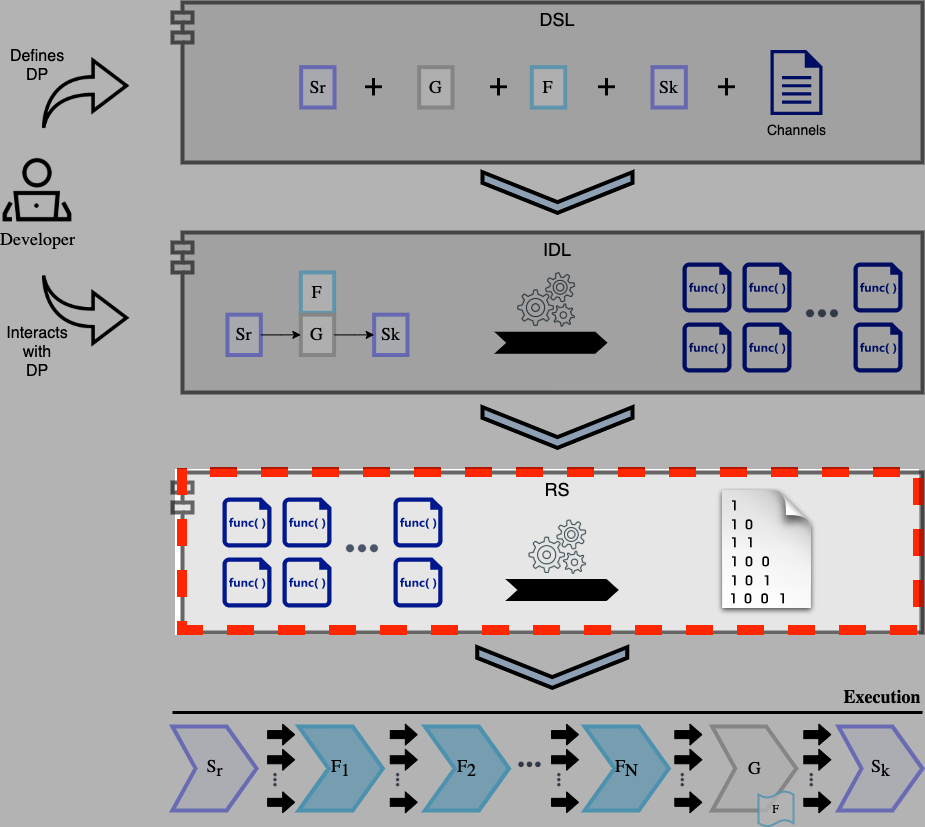
\includegraphics[width = 0.8\textwidth, height = 0.8\textheight]{dpf_haskell_v3-3}
    \end{center}
  \end{frame}

  \begin{frame}[fragile]{DP Haskell Framework}
    \begin{block}{Runtime System}
      \begin{itemize}
        \item \textbf{DP Monad}:
        \begin{itemize} 
        \item Monad with Existential Type to not escape DP Context. (\textit{Rank-2 Polymorphic type})
        \item Associativity Monad law guarantees execution flow (\mintinline{haskell}{ source >>= generator >>= sink }) 
        \end{itemize}
      \end{itemize}
    \end{block}
    \end{frame}
  
  \begin{frame}[fragile]{DP Haskell Framework}
    \begin{block}{Runtime System}
      \begin{itemize}
        \item \textbf{DP Monad}:
        \begin{itemize} 
        \item Monad with Existential Type to not escape DP Context. (\textit{Rank-2 Polymorphic type})
        \item Associativity Monad law guarantees execution flow (\mintinline{haskell}{ source >>= generator >>= sink }) 
        \end{itemize}
        \item \textbf{Filter / Stage}: 
        \begin{itemize}
          \item Use of \mintinline{haskell}{unfold} to generate dynamic filter computations (\textit{Anamorphism})
          \item Use of \mintinline{haskell}{fold} to reduce results to Sink (\textit{Catamorphism})
        \end{itemize}
      \end{itemize}
    \end{block}
    \end{frame}
  
  \begin{frame}[fragile]{DP Haskell Framework}
    \begin{block}{Runtime System}
      \begin{itemize}
        \item \textbf{DP Monad}:
        \begin{itemize} 
        \item Monad with Existential Type to not escape DP Context. (\textit{Rank-2 Polymorphic type})
        \item Associativity Monad law guarantees execution flow (\mintinline{haskell}{ source >>= generator >>= sink }) 
        \end{itemize}
        \item \textbf{Filter / Stage}: 
        \begin{itemize}
          \item Use of \mintinline{haskell}{unfold} to generate dynamic filter computations (\textit{Anamorphism})
          \item Use of \mintinline{haskell}{fold} to reduce results to Sink (\textit{Catamorphism})
        \end{itemize}
        \item \textbf{Multithreading}: \mintinline{shell}{async} library
      \end{itemize}
    \end{block}
    \end{frame}
  
  \begin{frame}[fragile]{DP Haskell Framework}
  \begin{block}{Runtime System}
    \begin{itemize}
      \item \textbf{DP Monad}:
      \begin{itemize} 
      \item Monad with Existential Type to not escape DP Context. (\textit{Rank-2 Polymorphic type})
      \item Associativity Monad law guarantees execution flow (\mintinline{haskell}{ source >>= generator >>= sink }) 
      \end{itemize}
    \item \textbf{Filter / Stage}: 
      \begin{itemize}
        \item Use of \mintinline{haskell}{unfold} to generate dynamic filter computations (\textit{Anamorphism})
        \item Use of \mintinline{haskell}{fold} to reduce results to Sink (\textit{Catamorphism})
      \end{itemize}
      \item \textbf{Multithreading}: \mintinline{shell}{async} library
      \item \textbf{Channels}: \mintinline{shell}{unagi-chan} library
    \end{itemize}
  \end{block}
  \end{frame}

  \begin{frame}[fragile]{DP Haskell Framework}
    \begin{center}
      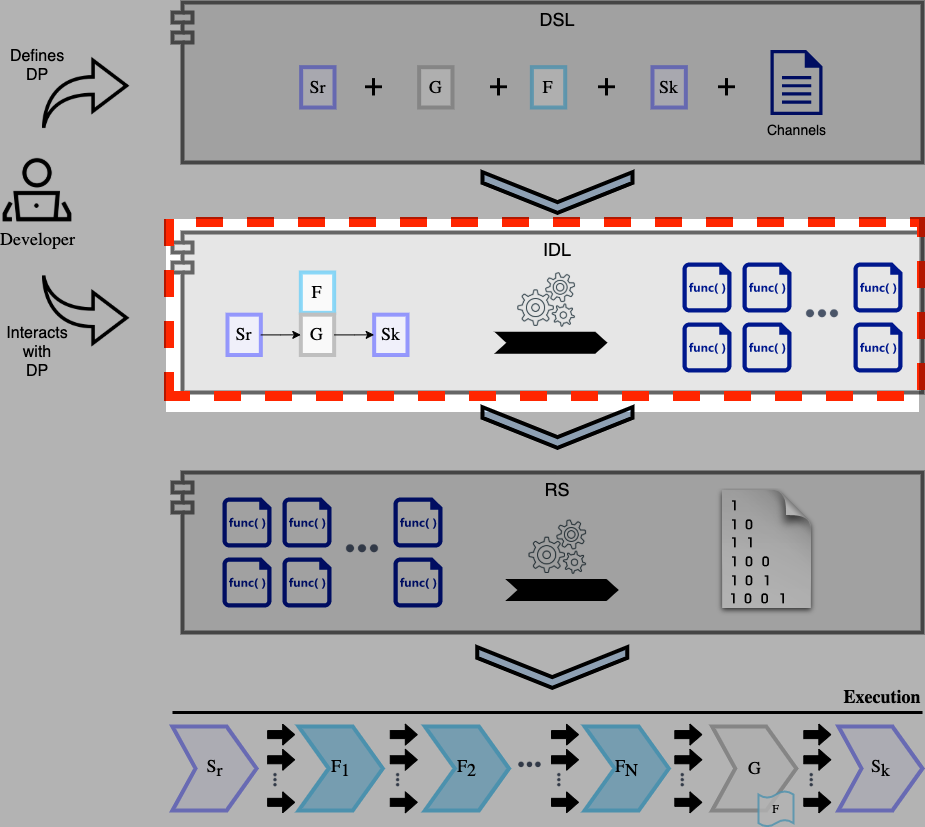
\includegraphics[width = 0.8\textwidth, height = 0.8\textheight]{dpf_haskell_v3-2}
    \end{center}
  \end{frame}

  \begin{frame}[fragile]{DP Haskell Framework}
    \begin{block}{IDL}
      \begin{minted}[fontsize=\small,breaklines]{shell}      
ghci> type DPExample = Source (Channel (Int :<+> Eof)) :=> Generator (Channel (Int :<+> Eof)) :=> Sink
type DPExample :: *
type DPExample =
  Source (Channel (Int :<+> Eof))
  :=> (Generator (Channel (Int :<+> Eof)) :=> Sink)
    \end{minted}
  \end{block}
  \end{frame}

  \begin{frame}[fragile]{DP Haskell Framework}
    \begin{block}{IDL}
      \begin{minted}[fontsize=\small,breaklines,highlightlines={7-11}]{shell}      
ghci> type DPExample = Source (Channel (Int :<+> Eof)) :=> Generator (Channel (Int :<+> Eof)) :=> Sink
type DPExample :: *
type DPExample =
  Source (Channel (Int :<+> Eof))
  :=> (Generator (Channel (Int :<+> Eof)) :=> Sink)
        
ghci> :t withSource @DPExample
withSource @DPExample
  :: forall k (st :: k).
      (WriteChannel Int -> DP st ())
      -> Stage (WriteChannel Int -> DP st ())
    \end{minted}
  \end{block}
  \end{frame}

  \begin{frame}[fragile]{DP Haskell Framework}
    \begin{block}{IDL}
      \begin{minted}[fontsize=\small,breaklines,highlightlines={7-9}]{shell}      
ghci> :t withSource @DPExample
withSource @DPExample
  :: forall k (st :: k).
      (WriteChannel Int -> DP st ())
      -> Stage (WriteChannel Int -> DP st ())
      
ghci> let source' = withSource @DPExample  $ \wc -> unfoldT ([1..10] <> [1..10]) wc identity
ghci> :t source'
source' :: forall k (st :: k). Stage (WriteChannel Int -> DP st ())
    \end{minted}
  \end{block}
  \end{frame}

  \begin{frame}[fragile]{DP Haskell Framework}
    \begin{block}{IDL}
      \begin{minted}[fontsize=\small,breaklines,highlightlines={2-8}]{shell}      
ghci> :t withGenerator @DPExample
withGenerator @DPExample
  :: forall k filter (st :: k).
      (filter -> ReadChannel Int -> WriteChannel Int -> DP st ())
      -> Stage
          (filter -> ReadChannel Int -> WriteChannel Int -> DP st ())    
    \end{minted}
  \end{block}
  \end{frame}

  \begin{frame}[fragile]{DP Haskell Framework}
    \begin{block}{IDL}
      \begin{minted}[fontsize=\small,breaklines,highlightlines={2-8}]{shell}      
ghci> :t withGenerator @DPExample
withGenerator @DPExample
  :: forall k filter (st :: k).
      (filter -> ReadChannel Int -> WriteChannel Int -> DP st ())
      -> Stage
          (filter -> ReadChannel Int -> WriteChannel Int -> DP st ())    
    \end{minted}
  \end{block}
  \begin{block}{Techniques}
    \begin{itemize}
      \item First Class Families
      \item Type-level Defunctionalization 
      \item Defunctionalization
      \item Associated Type Families
    \end{itemize}
  \end{block}
  \end{frame}

  \begin{frame}[fragile]{DP Haskell Framework}
    \begin{block}{}
      Library released on Hackage \\
      https://hackage.haskell.org/package/dynamic-pipeline
      \begin{center}
        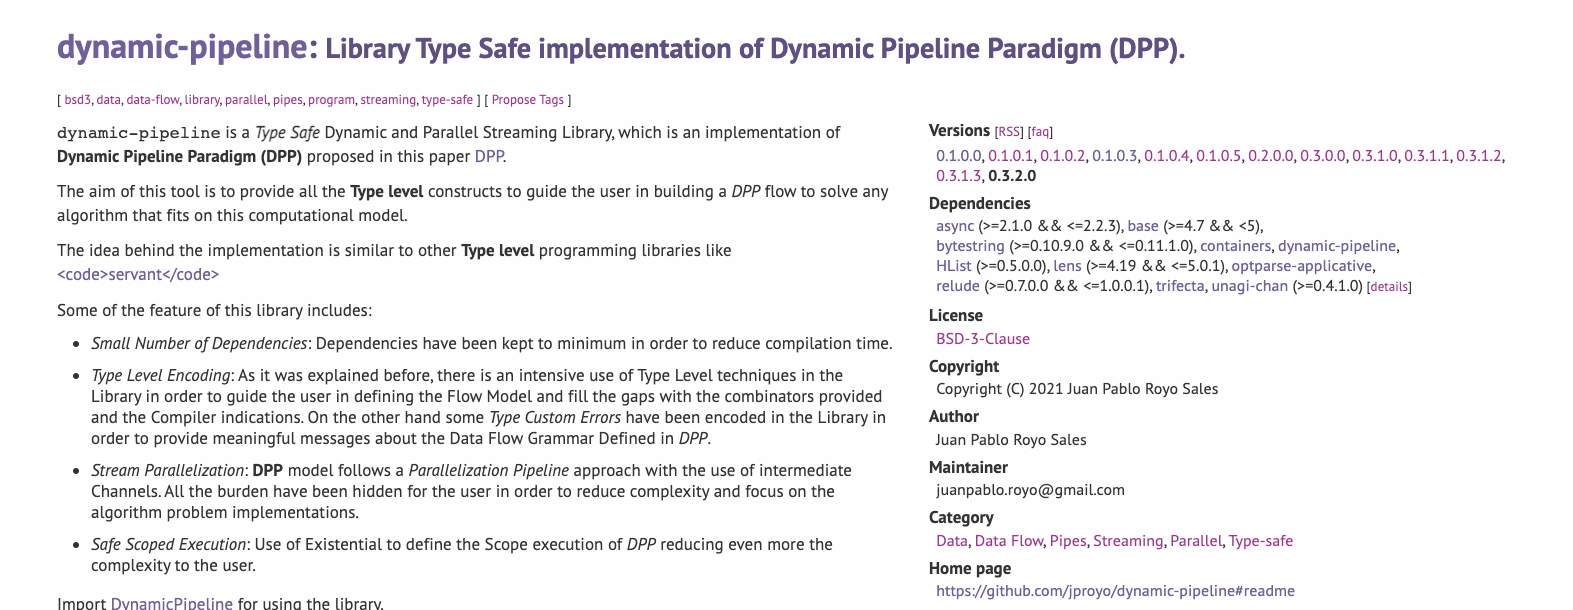
\includegraphics[width = 0.9\textwidth, height = 0.6\textheight]{dp-fw-hs}
      \end{center}  
    \end{block}
  \end{frame}

  \begin{frame}{Agenda}
    \section{Algorithm for Incrementally Enumerating BT in BG}
    \tableofcontents[currentsection]
  \end{frame}

  \begin{frame}[fragile]{Algorithm for Incrementally Enumerating BT in BG}
    \begin{block}{Program}
    \end{block}
  \end{frame}


  \begin{frame}{Agenda}
    \section{Empirical Evaluation}
    \tableofcontents[currentsection]
  \end{frame}


  \begin{frame}[fragile]{Empirical Evaluation}
    \begin{block}{Research Questions}
      \begin{itemize}
            \item Does $\dpwcc$ in Haskell support the dynamic parallelization level that $\dpwcc$ requires?
            \item Is $\dpwcc$ in Haskell competitive compared with default implementations on base libraries for the same problem?
            \item Does $\dpwcc$ in Haskell handle memory efficiently?
        \end{itemize}        
    \end{block}
    \begin{block}{Experiments}
      \begin{itemize}
        \item \textbf{Implementation Analysis}: Measure and analyze Total execution time, MUT time and GC Time.
        \item \textbf{Benchmark Analysis}: Compare $DP_{WCC}$ with \mintinline{haskell}{Data.Graph} $WCC$ execution times:
        \begin{itemize}
          \item Using \mintinline{haskell}{ criterion } library.
          \item Diefficency metric $\mathtt{dief@t}$ (\textit{diepfy} tool) to measure incremental results.
        \end{itemize}
        \item \textbf{Performance Analysis}: Thread and Memory allocation analysis.
      \end{itemize}
    \end{block}
  \end{frame}

  \begin{frame}[fragile]{Empirical Evaluation}
    \begin{block}{Graphs Tested}
    \begin{table}[H]
      \centering
      \begin{tabular}{|p{0.25\linewidth}|r|r|r|p{0.25\linewidth}|}
       \hline
       \textbf{Network} & \textbf{Nodes} & \textbf{Edges} & \textbf{\#WCC} & \textbf{\#Nodes Largest WCC} \\
       \hline
       Enron Emails & 36692 & 183831 & 1065 & 33696 (0.918) \\
       \hline
       Astro Physics Collaboration Net & 18772 & 198110 & 290 & 17903 (0.954)\\
       \hline
       Google Web Graph & 875713 & 5105039 & 2746 & 855802 (0.977)\\
       \hline
      \end{tabular}
     \end{table}
    \end{block}
    \begin{block}{Hardware Environment}
      \begin{itemize}
            \item $x86$ $64$ bits
            \item $6$-Core Intel Core i7 processor of $2,2$ GHz up to $12$ virtual cores
            \item \emph{Hyper-threading} enable
            \item $32 GB$ \emph{DDR4} of RAM, $256\ KB$ of L2 cache memory, and $9\ MB$ of L3 cache
        \end{itemize}        
    \end{block}
  \end{frame}

  \begin{frame}[fragile]{Empirical Evaluation}
    \frametitle{Diefficiency Metrics}
      \begin{figure}[!htb]
        \centering
        \begin{minipage}{0.33\textwidth}
         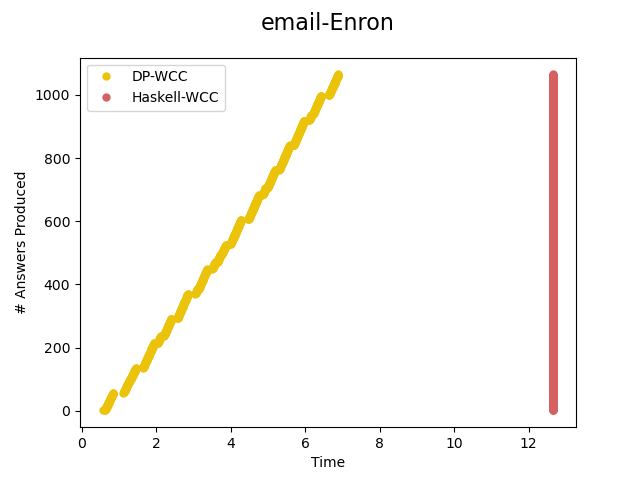
\includegraphics[width=1\linewidth, height=0.4\textheight]{email_enron}
        \end{minipage}%
        \begin{minipage}{0.33\textwidth}
         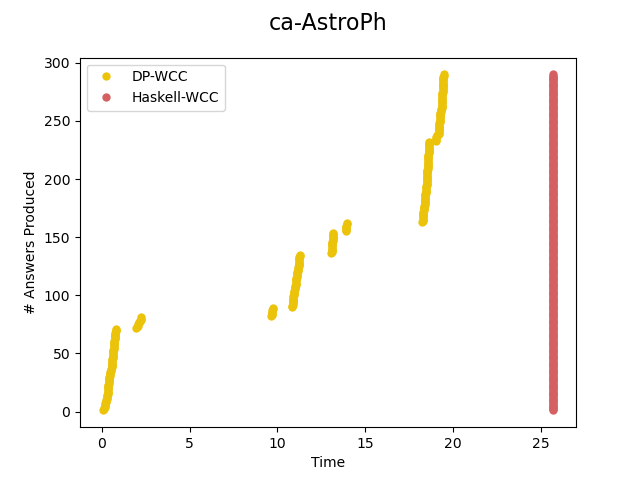
\includegraphics[width=1\linewidth, height=0.4\textheight]{ca_astroph}
        \end{minipage}%
        \begin{minipage}{0.33\textwidth}
         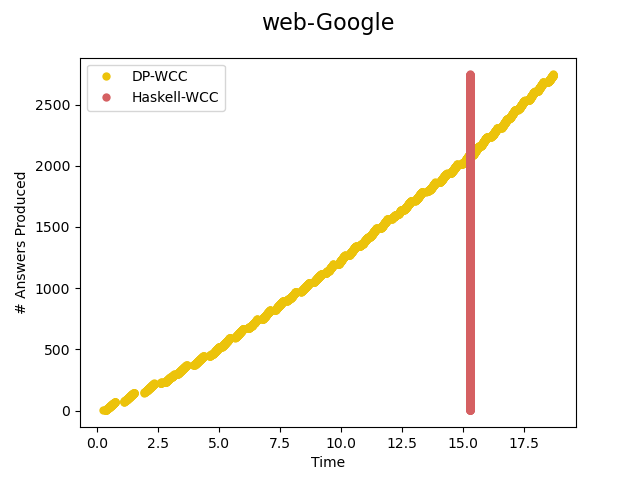
\includegraphics[width=1\linewidth, height=0.4\textheight]{web_google}
        \end{minipage}
    \end{figure}
  \begin{figure}[!htb]
      \centering
      \begin{minipage}{0.33\textwidth}
       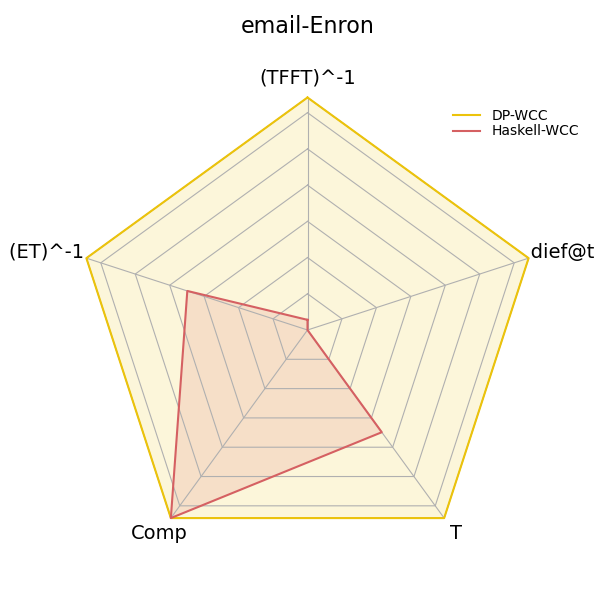
\includegraphics[width=1\linewidth, height=0.35\textheight]{email_enron_radar}
      \end{minipage}%
      \begin{minipage}{0.33\textwidth}
       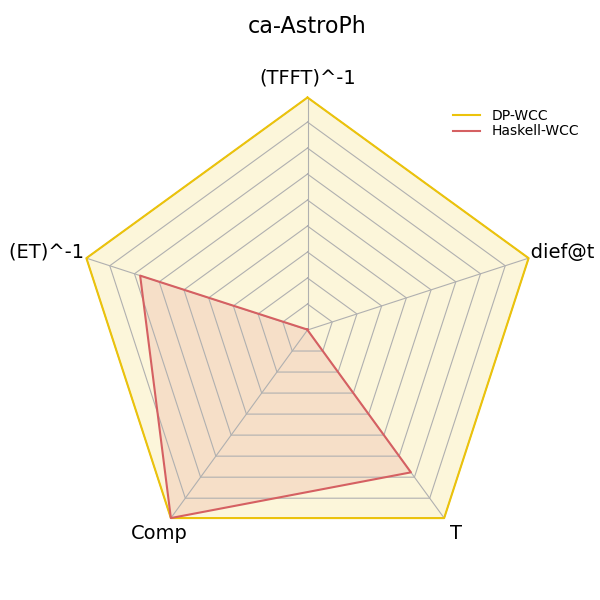
\includegraphics[width=1\linewidth, height=0.35\textheight]{ca_astroph_radar}
      \end{minipage}%
      \begin{minipage}{0.33\textwidth}
       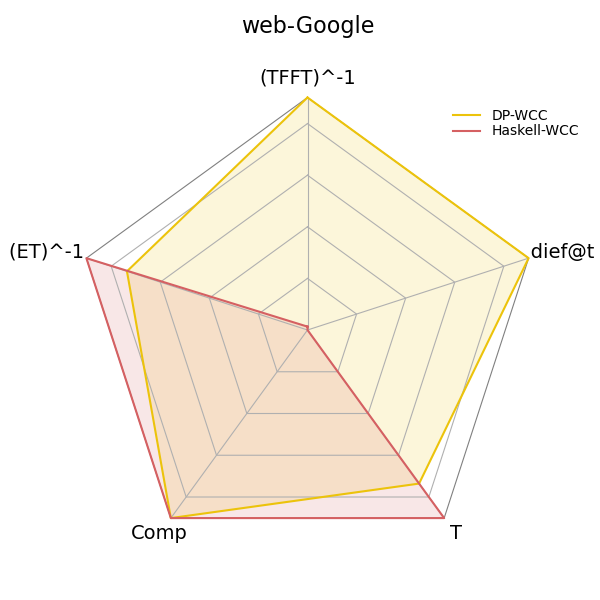
\includegraphics[width=1\linewidth, height=0.35\textheight]{web_google_radar}
      \end{minipage}
  \end{figure}
  \end{frame}

  \begin{frame}[fragile]{Empirical Evaluation}
    \frametitle{Benchmark}

    \begin{block}{Execution time}
    \begin{table}[H]
      \centering
      \begin{tabular}{|l|l|l|l|}
       \hline
       \textbf{Network} & \textbf{DP-Haskell} & \textbf{Data.Graph} & \textbf{Speed-up}\\
       \hline
       Enron Emails & 4.68s &  6.46s & 1.38\\
       \hline
       Astro Physics Coll Net & 4.98s & 6.95s  & 1.39\\
       \hline
       Google Web Graph & 386s & 106s & \color{red}0.27\\
       \hline
      \end{tabular}
     \end{table}      
    \end{block}

     \vspace{1cm}

    \begin{minipage}[t]{\linewidth}
      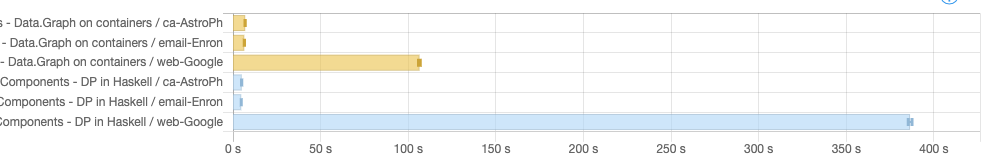
\includegraphics[width=\textwidth]{bench_2}
    \end{minipage}
  \end{frame}

  \begin{frame}[fragile]{Empirical Evaluation}
    \begin{columns}[onlytextwidth] 
      \begin{column}{.45\textwidth} 
        \begin{block}{ThreadScope}
          \begin{minipage}{\textwidth}
            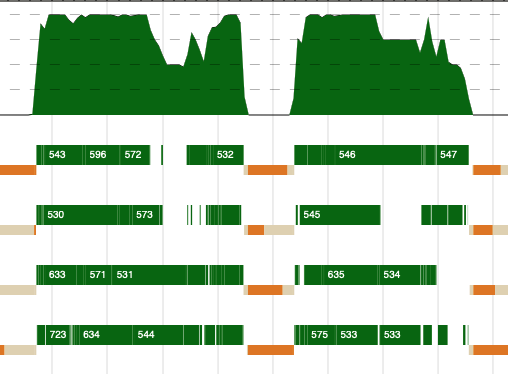
\includegraphics[width=1\linewidth, height=0.5\textheight]{screen_2}
          \end{minipage}%     
        \end{block}%
      \end{column} \hfill%
      \begin{column}{.45\textwidth} 
        \begin{block}{Eventlog - Memory Allocation}
          \begin{minipage}{\textwidth}
            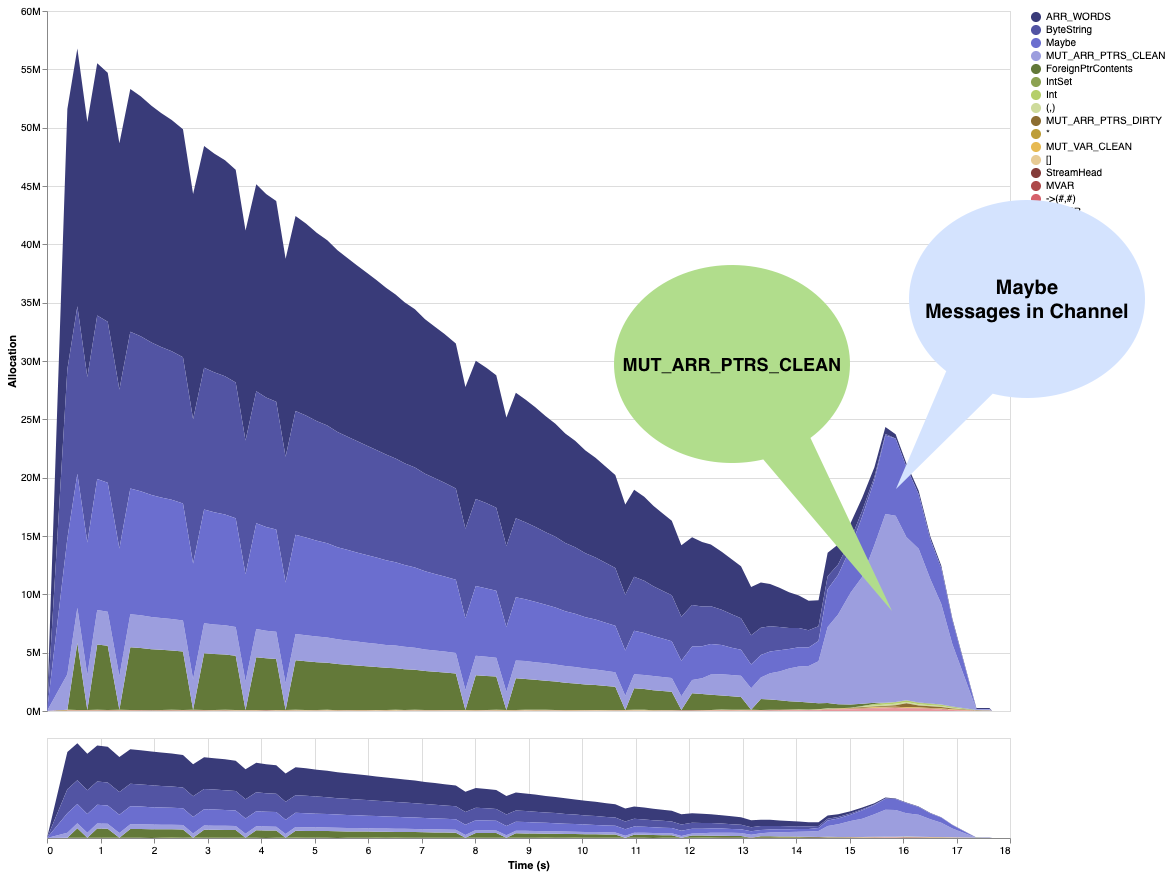
\includegraphics[width=1\linewidth, height=0.5\textheight]{visualization}
          \end{minipage}%
        \end{block}
    \end{column} 
  \end{columns}
  \end{frame}

  \begin{frame}{Agenda}
    \section{Conclusions and Future Work}
    \tableofcontents[currentsection]
  \end{frame}

  \begin{frame}[fragile]{Conclusions and Future Work}
    \begin{block}{Conclusions}      
      \begin{itemize}
        \item \textbf{Robustness and Suitability} of the DP-Haskell 
      \end{itemize}
    \end{block}
  \end{frame}

  \begin{frame}[fragile]{Conclusions and Future Work}
    \begin{block}{Conclusions}      

    \begin{itemize}
      \item \textbf{Robustness and Suitability} of the DP-Haskell 
      \item \textbf{Ability to generate Incremental results} has been shown by $\mathtt{dief@t}$ metrics 
    \end{itemize}
  \end{block}
  \end{frame}

  \begin{frame}[fragile]{Conclusions and Future Work}
    \begin{block}{Conclusions}      

    \begin{itemize}
      \item \textbf{Robustness and Suitability} of the DP-Haskell 
      \item \textbf{Ability to generate Incremental results} has been shown by $\mathtt{dief@t}$ metrics
      \item \textbf{Satisfactory Performance results} with an adequate Memory allocation and Execution times. 
    \end{itemize}
  \end{block}
  \end{frame}

  \begin{frame}[fragile]{Conclusions and Future Work}
    \begin{block}{Future work}      
    \begin{itemize}
      \item \textbf{Explore other Algorithms} to be implemented with this Paradigm.\footnote{We are currently working on Bi-partite Graphs algorithms}
      \item \textbf{Improve DP Framework} implementing more combinators and abstractions to allow the user write better and faster programs.
    \end{itemize}
  \end{block}
  \end{frame}

  \begin{frame}[allowframebreaks]
    \frametitle{References}
    \bibliographystyle{amsalpha}
    \bibliography{Report.bib}
  \end{frame}

  \begin{frame}
    \centering \Huge
    \emph{Questions?}
  \end{frame}  
  
\end{document}